\documentclass{article}
\usepackage[utf8]{inputenc}
\usepackage[russian]{babel}   % Подключение модуля для русского языка
\title{Конспект лекций И.А. Халидова по Теории Функции Комплексной переменной}
\author{Григорий Ефимов}
\date{Сентябрь - Декабрь 2021}
\usepackage{mathtools}
\usepackage{graphicx}
\graphicspath{{img/}}
\DeclareGraphicsExtensions{.pdf,.png,.jpg}
\begin{document}
    \begin{titlepage}
      \maketitle
    \end{titlepage}
    \tableofcontents
    \newpage
    \section{Введение}
        \subsection{Литература}
            \begin{itemize}
                \item Аксенов ТФКП
                \item Волькер Задачник
            \end{itemize}
            \newpage
        \subsection{Как устроены комплексные числа}
            \begin{equation}\label{eq:algebraik_form_complex}
                z=x+iy\footnotemark
            \end{equation}
            \footnotetext{ $i=-1$ }
            \begin{equation}\label{eq:algebraik_form_complex_w}
                w=u+iv
            \end{equation}
            Формула \ref{eq:algebraik_form_complex} - представление комплексного числа в алгебраическом виде. $x=Re(z)$ - вещественная часть комплексного числа (англ. real) $y=Im(z)$ - мнимая часть комплексного числа (англ. imagine)\\
            \begin{equation}\label{eq:exponential_form_complex}
                z=re^{i\phi}
            \end{equation}
            \begin{equation}\label{eq:trigonometric_form_complex}
                z=r(cos(\phi)+i sin(\phi))
            \end{equation}
          Формула \ref{eq:exponential_form_complex} - представление комплексного числа в показательной, формула         \ref{eq:trigonometric_form_complex} - в тригонометрической форме.\\
            Z \footnote{Часто множество комплексных чисел обозначают $C$, но мы так делать не будем, так как это обозначение сопадает с множеством непрерывных функкций} - множество комплексных чисел, т.е. комплексная плоскость. Если задаётся несколько плоскостей, то вторая задаётся буквой W и форумула \ref{eq:algebraik_form_complex_w} соответственно.
            \begin{equation}\label{eq:сomplex_module}
                |z|=sqrt(x^2+y^2)
            \end{equation}
            Модуль комплексного числа определяется по формуле \ref{eq:сomplex_module}
            \begin{figure}[h]
                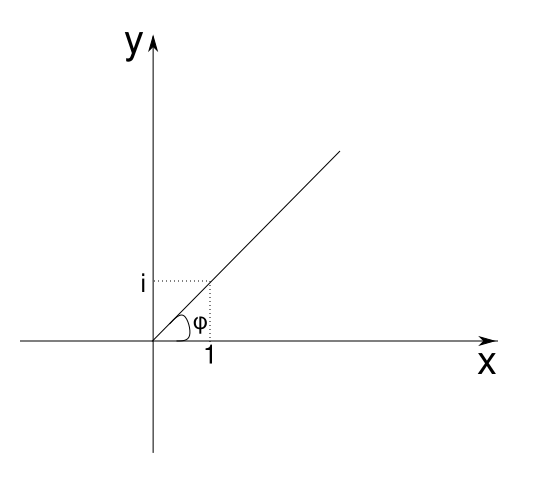
\includegraphics[width=0.6\linewidth]{complex_example}
                \caption{Графическое представление комплексного числа}
                \label{ris:complex_example}
            \end{figure}
              \begin{equation}\label{eq:complex_polar_example_x}
                  |z|cos(\phi)=x
              \end{equation}
              \begin{equation}\label{eq:complex_polar_example_y}
                  |z|sin(\phi)=y
              \end{equation}
            Формулы \ref{eq:complex_polar_example_x} и \ref{eq:complex_polar_example_y} нужны для представления полярного угла, являющегося $arg(z) $
            при этом важно, что $arg(z) \neq arctg(y/x)$, т.к. это корректно только для положительной полуплоскости
            \begin{equation}\label{eq:Arg_z}
                Arg(z)=\phi+2 \pi n
            \end{equation}
            Формуле \ref{eq:Arg_z} - формула аргумента уомплексного числа, т.е. множества чисел, отстоящих друг от дргуа на $2 \pi$, важно что Arg пишется с большой буквы. $arg(z)$ - главное значение аргумента, 
            \begin{math} 
              arg(z) \in 
              \begin{cases}
                [0;2 \pi] ($по учебнику$)\\
                [-\pi;\pi] ($этот вариант предпочтительней \footnotemark $)
              \end{cases} 
            \end{math}\\
            \footnotetext{Удобнее работать с чётностью, разрыв z будет в отрицательной полуплоскости, а в ней работают в реальных задачах реже}
            Комплексные числа работают с алгебраическими операциями и сохраняют свойства ассоциативности, дистрибутивности и комутативности.\\
            \begin{equation}\label{eq:Arg_z}
                z_{1} \pm z_{2}=(x_{1} \pm x_{2}) + i (y_{1} \pm y_{2})
            \end{equation}
          Сложение комплексных чисел в алгебраической форме\footnote{В полярной системе складывать комплексные числа сложнее сложнее}
            \begin{figure}[h]
                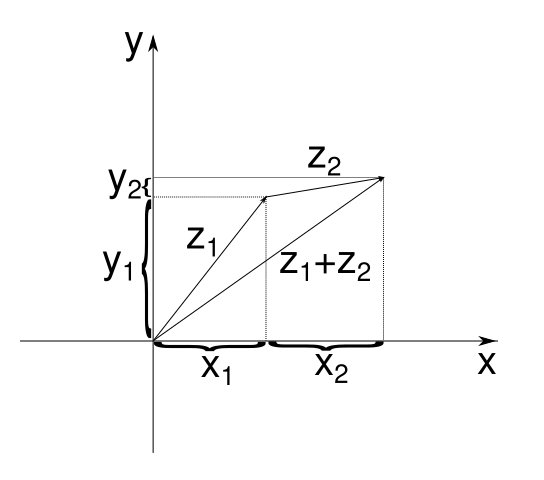
\includegraphics[width=0.8\linewidth]{adding_example}
                \caption{Графическое представление сложения двух комплексных чисел}
                \label{ris:adding_example}
            \end{figure}
            \begin{equation}
               z_{1} \cdot z_{2}=r_{1} r_{2} e^{i (\phi_{1} + \phi_{2})}              
            \end{equation}
            Уножение комплексных чисел в показательной форме\footnote{Для умножения удобнее использовать показательную, а не албебраическую форму}. Аналогично и с делением:
            \begin{equation}
               \frac{z_{1}}{z_{2}}=\frac{r_{1}}{r_{2}} e^{i (\phi_{1} - \phi_{2})}              
            \end{equation}
          Возведение в степень:
            \begin{equation}
               z=r^{n} e^{i n \phi}              
            \end{equation}
            $ \overline{z} $, иногда $z^{*}$ - комплексно-сопряженное число\footnote{Точка отражается относитеьно вещественной оси}, определим z из формулы \ref{eq:algebraik_form_complex}, тогда:
            \begin{equation}\label{complex_conjugate}
               \overline{z}=x-i y              
            \end{equation}
            \begin{equation}\label{complex_conjugate}
               \overline{z_{1} \pm z_{2}}=\overline{z_{1}} \pm \overline{z_{2}}              
            \end{equation}
            \begin{equation}\label{complex_conjugate}
               \overline{z_{1} \cdot z_{2}}=\overline{z_{1}} \cdot \overline{z_{2}}              
            \end{equation}
            С помощью комплексно-сопряжённых чисел можно делить комплексные числа в алгебраической форме:
            \begin{equation}
               \frac{ z_{2} }{ z_{1} } = \frac{ z_{2} \cdot \overline{ z_{1} }}{ \overline{z_{1}} \cdot z_{1} }
            \end{equation}
            \begin{equation}
               z \cdot \overline{z}=|z^{2}|
            \end{equation}
          Извлечение корня n степени из комплексного числа\footnote{Важно что Arg(z) - с большой буквы, т.к. значение не одно}, $n \in N $
            \begin{equation}
              \sqrt[n]{z}=\sqrt[n]{r} e^{\frac{i}{n} Arg(z)}=\sqrt[n]{r} e^{\frac{i}{n} \phi + 2 \pi k}
            \end{equation}
          Получается n корней, т.к. $\frac{2 \pi k}{n}$ имеет период n, и значения начнут повторяться. В точке 0 и в $\infty$ \footnote{
              В вещественных числах существует $+ \infty$ и $- \infty$, а у комплексных чисел есть только z=$\infty$, в неё можно попасть любым путём.
            } аргумент не определён
            \newpage
        \section{Стереографическая проекция}
\end{document} 
